% FIXME: Need reference
As seen from snapshots...the fluctuations can be quite strong, something which has also been observed experimentally.
This is in fact something which should be taken into account when modelling the plasma.
% FIXME: Need reference
Models like Hasegawa-Wakatani are doing a split between background and fluctuations.
There, the free energy in the background gradients are driving the fluctuations, and only the fluctuations are kept track of.
As long as the background fluctuations are not severely altering the background gradients, this is a good approximation.
On the other hand, when the background gradients are perturbed sufficiently by the perturbations, the drive for the fluctuations are also altered, and the fixed background approximation breaks down.
% FIXME: Need reference
Models like CYTO and CELMA does not do the separation of background and fluctuations, and one are with these models able to investigate how the fluctuations affect the background and not only the other way around.
We can do so by comparing the steady state profiles with the turbulent profiles.
A poloidal average and a temporal average containing the whole time series are done in order to get a good avergaged picture of the turbulent profile.
As apparent from figure \cref{fig:posOfFluct008} the background profiles are flattened by the turbulence.
%
\begin{figure}[htb]
    \centering
    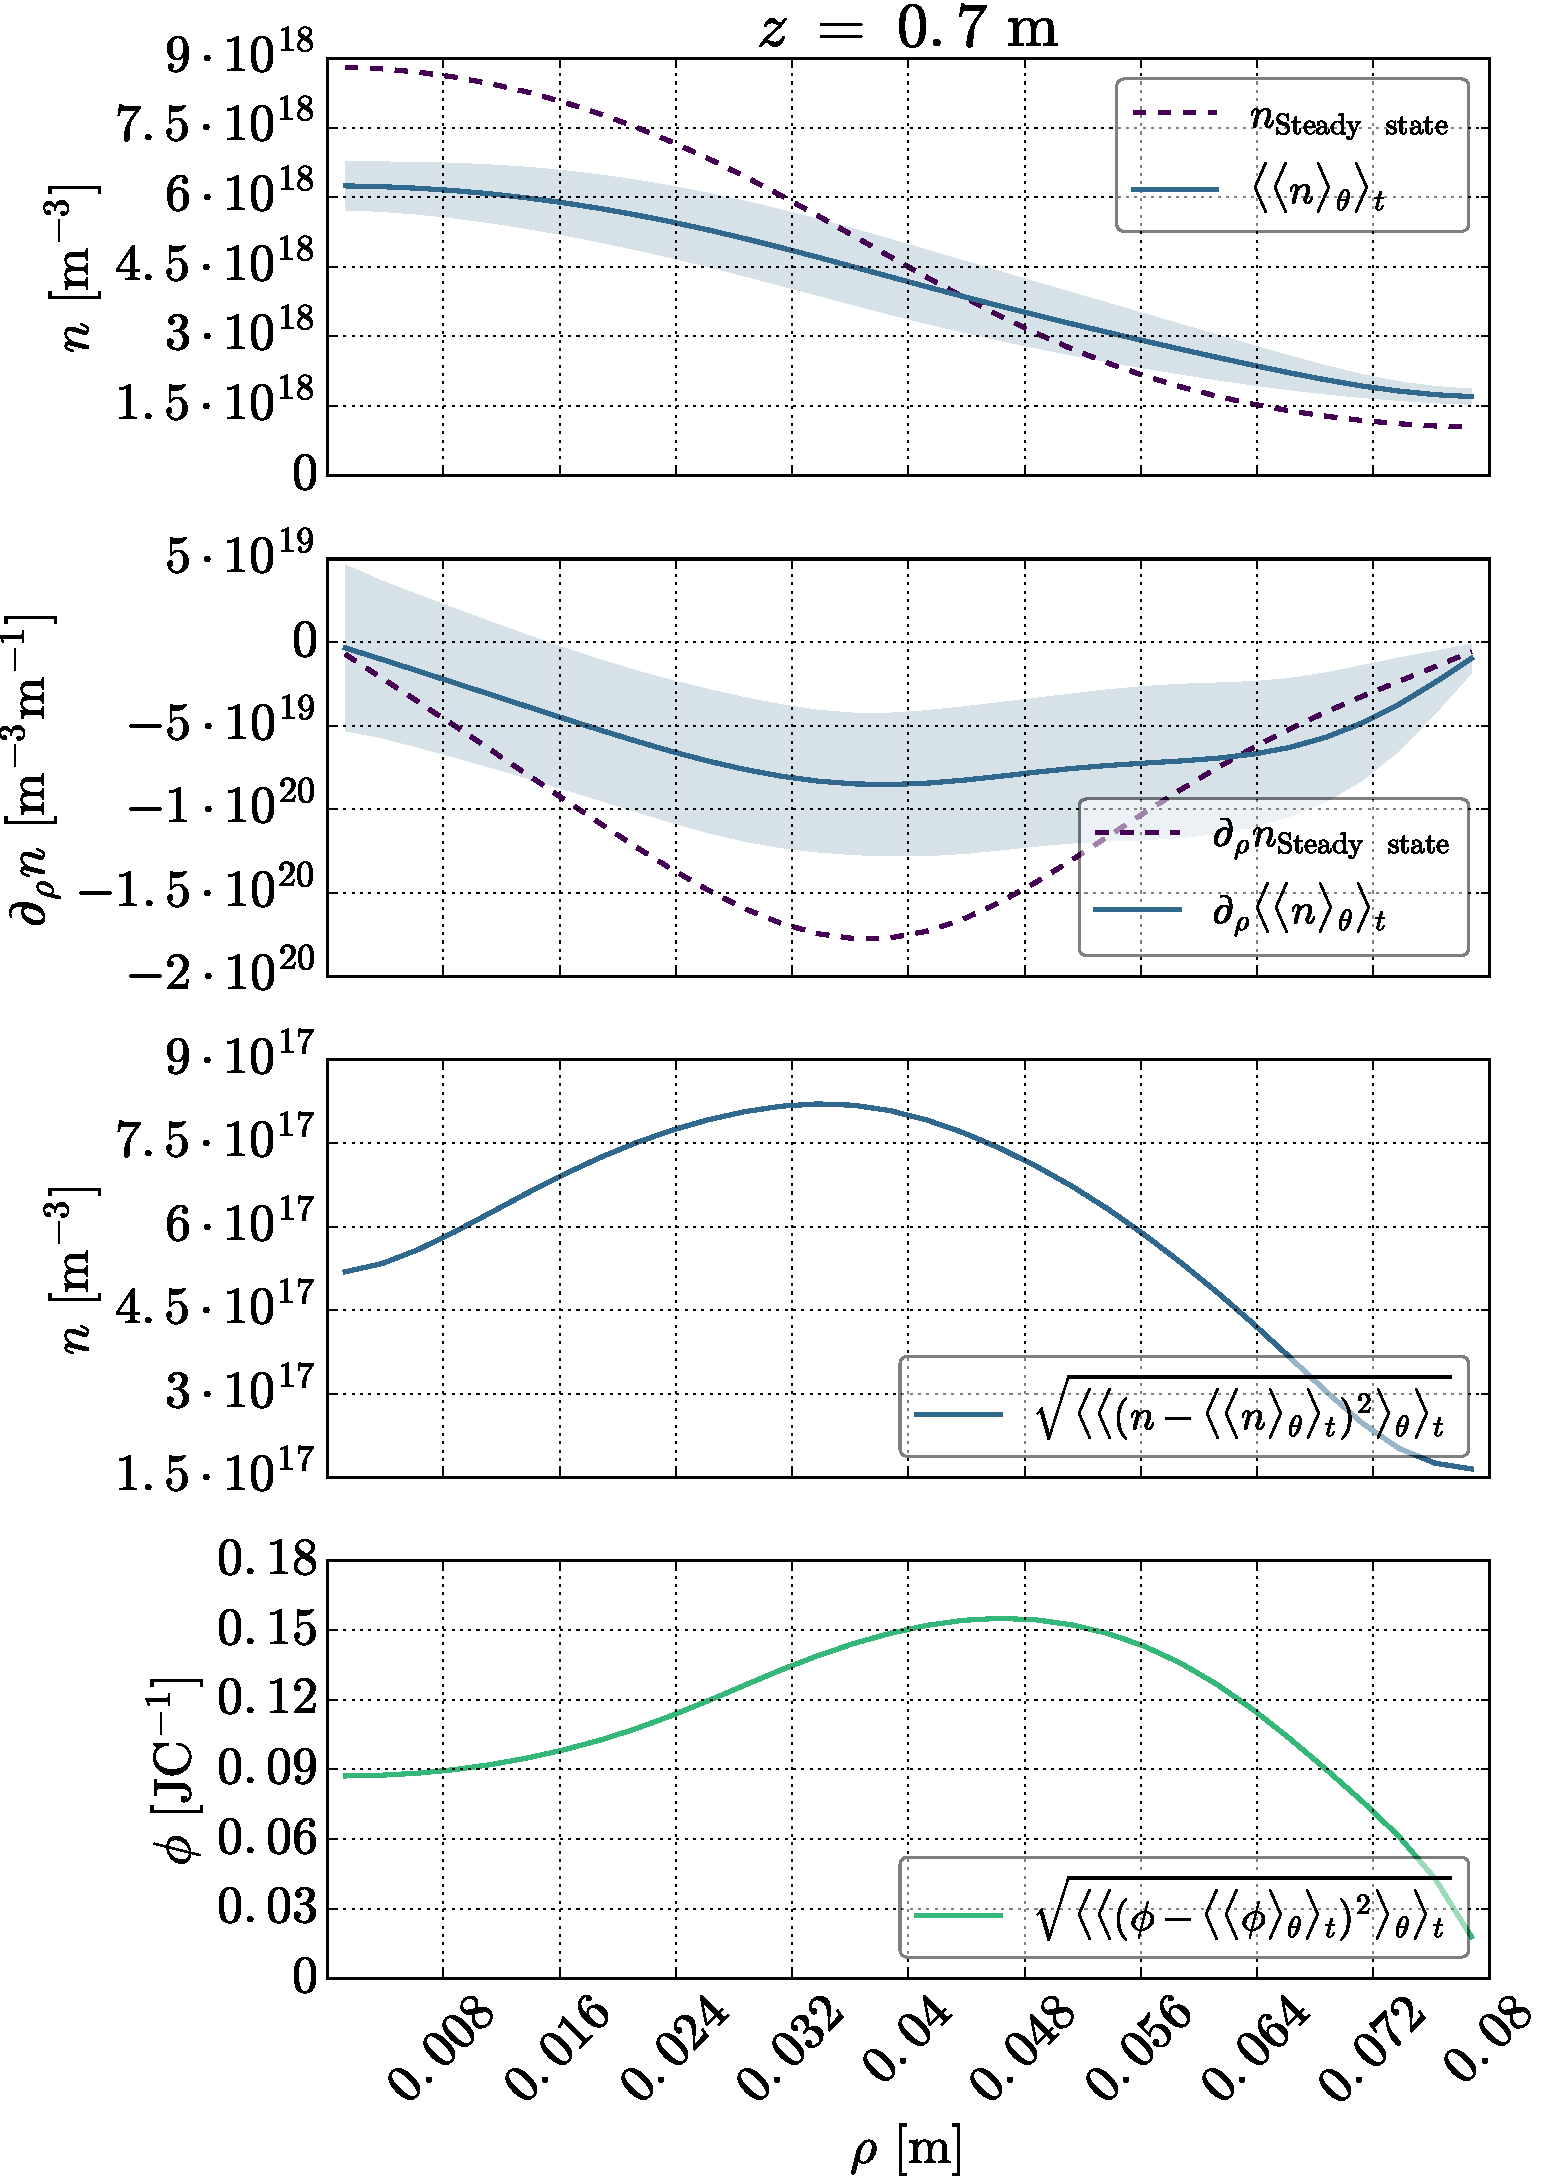
\includegraphics[width=0.5\textwidth]{fig/results/posOfFluct/posOfFluctB008}
    \caption{Flattening of the profiles together with the position of the fluctuations for $B=0.08\T$.
        The shaded area represents the standard deviation.
    }
    \label{fig:posOfFluct008}
\end{figure}
%

FIXME: Consider to include the type of fluctuation present.
Mention Jassby position of fluctuations.
NOTE: INSERT LINEAR THEORY AND LOCATION OF FLUCTUATIONS


Further investigation of the turbulence can be done through investigation of the time traces.
%
\begin{figure}[htb]
    \centering
    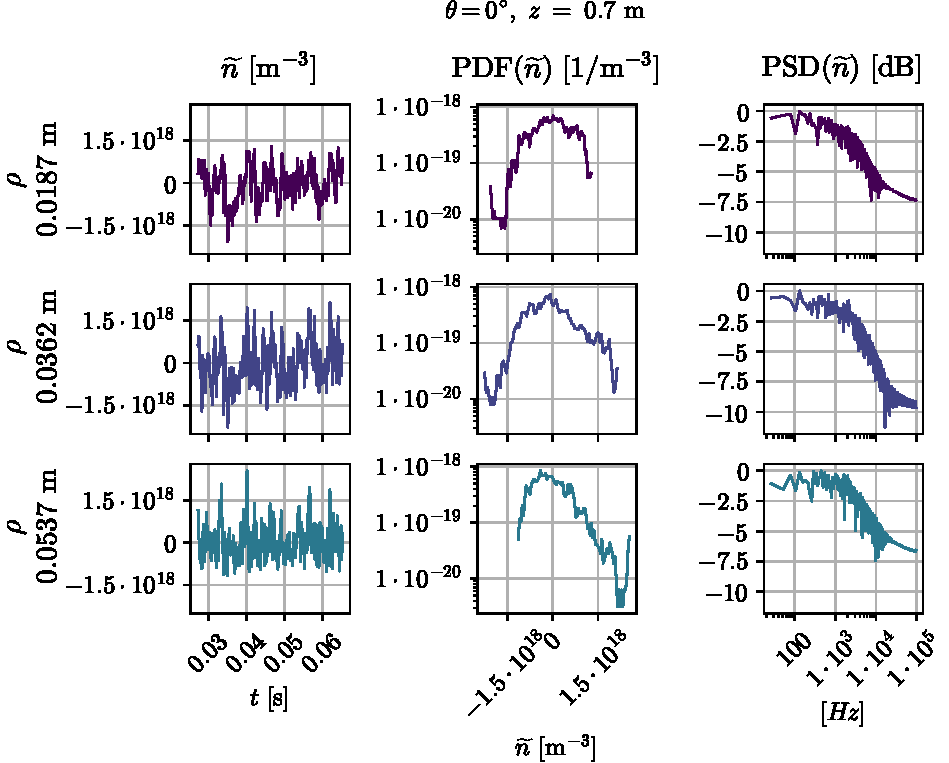
\includegraphics[width=1.0\textwidth]{fig/results/combinedPlots/008T}
    \caption{Characteristics of the time traces of the fluctuations at three radial positions.}
    \label{fig:combinedPlots008}
\end{figure}
%
This is done in \cref{fig:combinedPlots008}.
Again, we can observe that the fluctuations are large in amplitude, and (from the power spectra density PSD) that several frequencies are present simultanously.
This behavior is captured by the probability density functions (PDF), which measures the chance to encounter a value within an infetesimal range, if a value at a random time is withdrawn from the time trace.
Consequentually, if all values are equally probable, the PDF will have a Gaussian shape.
Deviations from the Gaussian shape is usually measured by the statistical moments skewness%
%
\footnote{
    The skewness is a measure of the mass of the distribution.
    If the skewness is negative, the left tail of the distribution is bigger than the right.
    For a pure Gaussian the skewness is 0.
}
%
and kurtosis
%
\footnote{
    The kurtosis is a measure of extreme events present in the distribution.
    For a pure Gaussian the skewness is 3.
    If the kurtosis is less than 3 (platykurtic) the distribution produces fewer and less extreme outliers than a gaussian.
    If the kurtosis is greater than 3 (leptokurtic) there are more extreme outliners, and the tails approaches zero slower than a Gaussian.
}
%
.
Figure \cref{fig:skewKurt008} highligths how this varies with the radius.
%
\begin{figure}[htb]
    \centering
    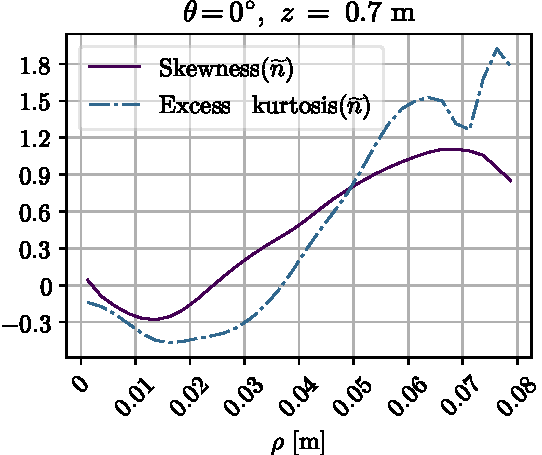
\includegraphics[width=0.5\textwidth]{fig/results/skewKurt/008T}
    \caption{Radial variations of the skewness and excess kurtosis (the kurtosis $-3$).}
    \label{fig:skewKurt008}
\end{figure}
%
One can see that close to the center, it is more probable to encounter a large negative fluctuation than a positive fluctuation.
Then, for higher radii, large positive fluctuations becomes more and more frequent.
From the excess kurtosis, we can see that extreme events are less likely than in a Gaussian random process, whereas extreme events are almost twice as likely in the edge as in a Gaussian random process.

Finally it can be noted that the radial turbulent transport is mainly positive and even more intermittent than the fluctuations in density alone.
